\chapter{Methods}

One of the motivations of using flip probability as a loss function is the 'cold start' problem in \gls{ml}. Ideally, one could 'warm start' a network by training it from scratch with a small sample. This is not dissimilar to the idea of \gls{dataaugmentation} - improving the ability of the network to learn on the raw data. This is a problem that is exacerbated further in the context of \gls{dl}, as there are many more millions of parameters (in modern networks) and hence the \gls{parameterspace} is much larger. One hypothesis is that one could use \gls{fp} to perform \gls{representationlearning} on less data than would usually be required so that the network will train quickly.

\begin{hypothesis} %\begin{hyp}[H\ref{hyp:first}] \label{hyp:first}
Using \gls{fp} to perform \gls{representationlearning} on the data will allow the network to train more quickly.https://www.overleaf.com/project/5d4c12731e8baf5a40f9c2d9
\label{hyp:first}
\end{hypothesis}

% this is something of a false dichotomy - need to investigate how CE performs around edges
Another problem with classifiers trained using a traditional loss function, like \gls{mse}, is that (as illustrated by figures \ref{fig:poor_sep_classes} and \ref{fig:good_sep_classes}) they tend to generalise poorly, especially when the data classes are closely spaced geometrically. Hence, by using \gls{fp} to find a representation of the data that spaces out these classes in a geometric sense, we might expect to see an increase in \gls{generalisationperformance}.

\begin{hypothesis} %\begin{hyp}[H\ref{hyp:first}] \label{hyp:first}
Using \gls{fp} to perform \gls{representationlearning} on the data will improve \gls{generalisationperformance}.
\label{hyp:second}
\end{hypothesis}

Another key idea, as mention in 

\section{Flip Probability}

We have some data:

\begin{equation}
X \in \mathds{R}^d 
\end{equation}

Where $d$, the dimensionality of the data, is quite high. \bigskip

For a single batch of data and a single classifier, the empirical flipping probability can be thought of as the proportion of label 'flips' that occur when the classifier and binary data are randomly projected down (using a \gls{rp} matrix) to a lower dimension:

\begin{equation}
P((R h)^T Rx \neq h^{T}x)  
\end{equation}

An example of a (linear) classifier is a single neuron in a \gls{nn} at the last layer. Randomly projecting the classifier and minimising the \gls{fp} can act as a proxy for learning a classifier in the projected space. \smallskip

\gls{fp} can then be defined empirically:

\begin{equation}
\hat{P}\ := \\ P(\frac{1}{m}\sum_{j = 1}^m (R_j h)^T R_{j}x \neq h_i^{T}x)  
\end{equation}

Where;  \smallskip

\begin{itemize}
\item $\hat{P}$ is the empirical estimate of the flipping probability  
\item $R$ is the \gls{rp} matrix  
\item $P$ is the proportion of inequalities recorded over the data 
\item $h_i$ is the classifier  
\end{itemize}

If  \gls{fp} is small, the points are well separated. \bigskip

The entries of $R$ are typically drawn from a normal distribution (and will be in this instance) but can also be drawn from other distributions in order to speed up generation of the random (projection) matrices while training the network:

\begin{equation}
R \in M^{kxd}, R_{ij} \stackrel{i.i.d}{\backsim} N(0,1) 
\end{equation}

When $d$ is very large, subgaussian random variables can be used replacements. One such alternative is the Rademacher discrete distribution:

\begin{equation}
R \in M^{kxd}, R_{ij} = \pm 1 \; w.p. 0.5 
\end{equation}

\begin{itemize}
\itemsep-1em 
\item $M$ is the number of classes  
\item $k$ is the projection dimension, a user specified parameter 
\item $R_{ij}$ is an individual entry of the \gls{rp} matrix  \gls{sgd}  
\end{itemize}

One example of $h_i$ is the ZAMBINGO at the $i^{th}$ node of the last layer of an \gls{mlp}. This would take the form of a vector of weights that are applied to (cross-multiplied with) the inputs from the previous layer and a bias term is added, before the \gls{activationfunction} for the layer is added.
\bigskip

\bigskip

\gls{fp} implemented using  \gls{sgd} would look like the following:

\begin{equation}
\label{eq:sgd_fp}
\hat{P}\ := \frac{1}{L}\frac{1}{M}\sum_{l = 1}^N \sum_{j = 1}^M \mathds{1}((R_j h_i)^T R_jx_L \neq h_i^Tx_L)  
\end{equation}

Where;  \smallskip

\begin{itemize}
\itemsep-1em 
\item $\mathds{1}$ is the \gls{indicatorfunction}  
\item $k$ is the projection dimension, a user specified parameter 
\item $R_{ij}$ is an individual entry of the \gls{rp} matrix  \gls{sgd} 
\item $x_L$ is the batch of data used during  \gls{sgd}  
\item $N$ is the number of batches of data used in  \gls{sgd}  
\item $M$ is the number of classes %is the number of \gls{rp} matrices
\end{itemize}

Equation \ref{eq:sgd_fp} fails to consider the possibility that the randomly projected classifier,  $(R_j h_i)$, will classify the data, $x_L$, correctly where the unprojected classifier has classified the data incorrectly.
\bigskip

\begin{equation}
\label{eq:conditional_sgd_fp}
\hat{P}\ := \frac{1}{L}\frac{1}{M}\sum_{l = 1}^N \sum_{j = 1}^M  \mathds{1}( (R_j h_i)^T R_jx_L \neq h_i^Tx_L \mid \hat{h_i^T}x_L = y_i )  
\end{equation}
%\myequation{Empirical Conditional Flip Probability for Stochastic Gradient Descent}

Where $y_i$ is the correct label of the data $x_i$. 
\bigskip

Equation \ref{eq:conditional_sgd_fp} correctly accounts for this (although it is anticipated with a well trained classifier, this situation would account for a negligible proportion of cases). 
\bigskip

How often the projected classifier incorrectly classifies the data when the data is compressed strongly depends on the geometry of the data. The key idea with using \gls{fp} as a loss function in a \gls{nn} context is to "drive the representation to a nice place" aka, undergo effective unsupervised representation learning before learning a classifier on the data. 
\bigskip

% TODO - more explain on FP

Implementing  \gls{fp} inevitably encounters a problem in that loss functions must be differentiable, if the network is to be trained using gradient descent, or a variant thereof (such as the \gls{adam} algorithm). In particular, the loss function must be differentiable with respect to the parameters of the model in order for the gradients to be backpropagated through the network. The gradients are then used to update the parameters in the correct direction (towards a local, and hopefully global, optimum). Modern tools incorporate auto-differentiation libraries to lessen the mathematical challenge of specifying derivatives for complex loss functions, but the function, when decomposed, must still nonetheless be differentiable.
\bigskip

Hence, a major challenge with the above loss functions is that they are not differentiable, primary due to the inequality involved. This inequality introduces a discontinuity in the function, which is not differentiable. One way to get around this is to recognise that in principle, we are minimising the angle between the data and the classifier \cite{}

\begin{equation}
\label{eq:sgd_fp}
\hat{FP}\ := \frac{1}{L}\frac{1}{M}\sum_{l = 1}^N \sum_{j = 1}^M \mathds{1}((R_j h_i)^T R_jx_L \neq h_i^Tx_L)  
\end{equation}
%\myequation{Empirical Flip Probability for Stochastic Gradient Descent}

\section{Implementation of Flip Probability}

To practically implement \gls{fp}, we return the input of



One way we can reduce the computational burden of this procedure is to generate the \gls{rp} matrices at the start of the algorithm instead of dynamically each time the loss function is called. This has the disadvantage of introducing dependencies \cite{bob_rp_storage}, but given the number of \gls{rp} matrices needed to be generated in even a small \gls{cnn}, this is a necessary step in order for testing and iteration to be feasible. 
\bigskip

\begin{algorithm}[H]
\SetAlgoLined
\KwResult{Write here the result }
 initialization\;
 \While{While condition}{
  instructions\;
  \eIf{condition}{
   instructions1\;
   instructions2\;
   }{
   instructions3\;
  }
 }
    \caption{The 10 fold \gls{cv} algorithm}
    \label{algo:fp_python_1}
\end{algorithm}

% TODO - calculate number of RP matrices need for static storage and dynamic generation
\section{Data sets}
 
%\subsection{Artificial Data}
%
%In order to test the effectiveness of \gls{fp} as a loss function, some %synthetic, linearly separable data was generated. As  \gls{fp} benefits %from the \gls{jll}, it was necessary to ensure this was sufficiently highly %dimensional. Hence, data with dimension $k =$ 5,10,20,50,100,500,1000,10000 %was generated to test with a  \gls{nn}. 
%\bigskip

 \subsection{MNIST}
 
\url{\gls{mnist}}{http://yann.lecun.com/exdb/mnist/} is a famous data set often regarded as a starting point to work on and experiment with. It represents an improvement over the older \gls{nist} data set, which used images from different sources (high school students and workers) for the training and testing set \cite{nist}. It comprises of images of handwritten digits (of ten classes, 0-9), scaled, centered and batch normalised into 28x28 grayscale images. Of 60k images, these are split into 10k training images and 50k testing images \cite{mnist}. This type of problem (digit recognition) is fairly unique in image classification in that the visual information directly conveys the \gls{classlabel}, i.e. there is a direct mapping between the image and the label. Modern training accuracies are sufficiently high (less than 0.2\%, \cite{mnist_sota}) on \gls{mnist} that it can be considered a 'solved' problem \cite{mnist_sota_web}. However, this data is of sufficientl dimensionality ($28 * 28 = \mathds{R}^{784}$) that it can adequately be used as a test for \gls{fp} in a \gls{cnn} context. 
 \bigskip

%\subsection{CIFAR-10}
%
%To extend upon the \gls{mnist} testing with a more challenging data set, %the ten class \gls{cifar}-10 data set was used. Here, the mapping between %image and label is less direct, and the complexity of the images (which %include animal and vehicles) is increased. These images are \gls{rgb} and %of 32x32. Hence, they have a dimension of $3 * 32 * 32 = %\mathds{R}^{3072}$. Because of this increased dimensionality, we include a %pooling layer and add an extra \gls{fc} layer to complexify the network.
%\bigskip

%Tiny ImageNet:
%
%Tiny ImageNet is smaller version of the well-known \gls{ilsvrc} ImageNet, %which has over a million images.

\section{Testing Schemes}
  
It is necessary to have baseline results to compare the performance of \gls{fp} against. While there are various data preprocessing (scaling, whitening), and \gls{dataaugmentation} strategies (e.g. flipping, cropping, rotation and jittering)  available, we use a fairly simple script in Pytorch (\cite{mnist_script}) that uses the test/train split present in the  \gls{mnist} data set and rapidly achieves an accuracy of 97\%. Ideally, we would test the algorithms using 10 fold-\gls{cv} (the 'gold standard', \ref{algo:10-fold-cv}). However, this introduces a high level of computational burden, as the algorithm must be run independently across at least 10 subsets of the data. This script was built upon by:

\begin{itemize}
    \itemsep-1em 
    \item Writing new \gls{lossfunction}s to implement \gls{fp}
    \item Configuring the network architecture to handle the new \gls{lossfunction}s
    \item Testing the new architecture and \gls{lossfunction} with a variety of \gls{hyperparameter} settings
    \item Simplifying the script to handle artificial data and complexifying the script to handle \gls{cifar}-10
\end{itemize}

The layers of the network trained on \gls{mnist} \footnote{\url{See Adam W. Harley's excellent \gls{mnist} visualisation}{https://www.cs.ryerson.ca/~aharley/vis/conv/} to explore the internals of how using a \gls{cnn} to classify digits works \cite{mnist_viz}.}

\begin{itemize}
    \itemsep-1em 
    \item Convolution layer 1 (Input layer) : 1,10
    \item Convolution layer 2 : 10,20
    \item (if Dropout enabled) Dropout layer 
    \item Fully Connected layer 1 : 320, 50
    \item Fully Connected layer 2 (Output layer) : 50, 10
\end{itemize}

To show the effect this has on the dimensionality of the data, see \ref{fig:cnn_mnist_dims}. 

% fig for cnn mnist dims

\bigskip

% ZAMBINGO - cv algorithm
\begin{algorithm}[H]
\SetAlgoLined
\KwResult{Write here the result }
 initialization\;
 \While{While condition}{
  instructions\;
  \eIf{condition}{
   instructions1\;
   instructions2\;
   }{
   instructions3\;
  }
 }
    \caption{The 10 fold \gls{cv} algorithm}
    \label{algo:10-fold-cv}
\end{algorithm}

% ZAMBINGO - insert diagram for cv here 
% https://cran.r-project.org/web/packages/groupdata2/vignettes/cross-validation_with_groupdata2.html

\bigskip

Instead, for a reasonable test of \gls{generalisationperformance}, we can use the typical test-train split, where 10\% of the data is used for testing and 90\% is used for training. This split is randomly determined.
\bigskip

In terms of \gls{hyperparameter} tuning, various modern methods for this exist, the simplest of which is the grid search. This also results in a high computational burden, being a brute force strategy. 
\bigskip

\begin{figure}
    \centering
    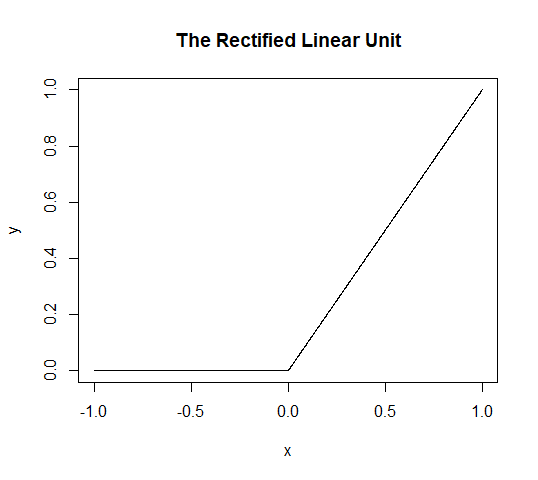
\includegraphics[scale=0.5]{figs/relu.png}
    \caption{The ReLu activation function.}[The ReLu activation function, also known as the 'hinge loss', known for it's ease of computation and efficacy in training networks.]
    \label{fig:relu_function}
\end{figure}

The \gls{relu} (figure \ref{fig:relu_function}) was used as the activation function in all testing schemes. This is an \gls{activationfunction} that is fast to compute, easy to interpret, widely used, and performs well in neural networks generally (\cite{activation_search}). 
\bigskip

% Zambingo - formatting is borked here
In all cases;

\begin{itemize}
    \itemsep-1em 
    \item Batch size = 64
    \item The optimisation method was \gls{sgd}
    \item The learning rate was 0.01
    \item Kernel size = 5
\end{itemize}

Where normalisation was performed, this was over each input channel \footnote{\url{https://pytorch.org/docs/stable/torchvision/transforms.html}}, using a mean of 0.1307 and a standard deviation of 0.3081, which are known to be the mean and standard deviation of the grayscale (only) channel of \gls{mnist}.

\begin{landscape}

%\newgeometry{left=0.5cm,top=0.5cm,bottom=0.5cm,right=0.5cm}

\begin{table}[hp]
    \centering
    \begin{tabular}{ |p{1cm}||p{1.5cm}|p{1cm}|p{1cm}|p{1cm}|p{1cm}|p{1cm}|p{6cm}| }
         \hline
         \multicolumn{8}{|c|}{Scheme Parameters} \\
         \hline
         No. & Epochs & $M$ & Loss & 2nd Loss & DO & $N$ & Notes\\
         \hline
         1 & 100 & - &FP &CE &0.5 &Y & Alt. Loss per batch\\
         2 &\cellcolor{blue!25} 10 & - &FP &CE &0.5 &Y & Alt. Loss per batch\\
         3 & 10 & - &FP &CE &\cellcolor{blue!25} - &Y & Alt. Loss per batch\\
         4 &\cellcolor{blue!25} 5 & -  &FP &CE & - &Y & Alt. Loss per batch\\
         5 & 10 & -  &FP &CE & - &Y & \cellcolor{blue!25}Alt. Loss over run\\
         6 & \cellcolor{blue!25}10 & \cellcolor{blue!25}0.5 &FP &CE & - &Y & Alt. Loss over run\\
         7 & \cellcolor{blue!25}20 & 0.5 &FP &CE & - &Y & Alt. Loss over run\\
         8 & 10 & 0.5 &FP &CE &0.5 &Y & \cellcolor{blue!25}Short FP periods, alternating\\
         9 & 10 & 0.5 &\cellcolor{blue!25}CE & - &0.5 &Y & Baseline\\
         10 & 10 & 0.5 &CE & - & - &\cellcolor{blue!25}N &Baseline - No Normalisation\\
         11 & 20 & - &FP &CE & - &Y & \cellcolor{blue!25}Switched loss at midpoint*\\
         12 & \cellcolor{blue!25}100 & - &FP &CE & -  &Y & Switched loss at midpoint*\\
         \hline
         \multicolumn{3}{@{}p{1.5in}}{\footnotesize (DO) $=$ Drop-out}\\
         \multicolumn{3}{@{}p{1.5in}}{\footnotesize ($M$) $=$ Momentum}\\
         \multicolumn{3}{@{}p{1.5in}}{\footnotesize ($N$) $=$ Normalisation}\\
         \multicolumn{3}{@{}p{1.5in}}{\footnotesize (-) $=$ Unused}\\
         \multicolumn{3}{@{}p{3in}}{\footnotesize (*) $=$ Keeping layers frozen as appropriate}\\
    \end{tabular}
    \caption{Testing Schemes run on MNIST. Coloured background indicate a change in parameters from the previous similar scheme.}
    \label{table:testing_schemes}
\end{table}

\end{landscape}

%\restoregeometry

\section{Hardware}

When benchmarking for running time, the \gls{nn}s were run on an Asus laptop with 8 \gls{gb}s of \gls{ram}, a Intel Core i5-8250U processor and a 256\gls{gb} \gls{ssd}. All operations were run on the \gls{cpu}. \href{https://colab.research.google.com/}{Google colaboratory}, a cloud notebook platform, was also used to run the networks. A collection of note 

\section{Software}

All networks were implemented in \href{https://pytorch.org/}{Pytorch}, a \gls{dl} platform built on top of the older 'torch' library. Python was used to design and run all code. Pytorch has the advantage of being more easily able to be modified at a low level, which is necessary for designing and integrating custom loss functions. It also has a 'pythonic' imperative style, which is less obtuse than the declarative style used in Tensorflow and the reductionist style of Keras \cite{tale_dl}. All code used to generate results and visualisations and latex written for this dissertation can be accessed at the \href{https://github.com/MattSkiff/Flip-Probability-as-a-Loss-Function-in-Convolutional-Neural-Networks-for-Image-Classification}{GitHub repository}. This document was written using \href{https://www.overleaf.com/}{Overleaf}. \href{https://inkscape.org/}{Inkscape} was used for non-programmatic diagrams.